\documentclass{article}
\usepackage[pdftex]{graphicx} %for embedding images
\usepackage{url} %for proper url entries
\usepackage[bookmarks, colorlinks=false, pdfborder={0 0 0}, pdftitle={Research Outline - Science Research Method}, pdfauthor={Le Nhut Nam}, pdfsubject={ntroduction to Machine Learning}, pdfkeywords={report, exercises}]{hyperref} %for creating links in the pdf version and other additional pdf attributes, no effect on the printed document
%\usepackage[final]{pdfpages} %for embedding another pdf, remove if not required
\usepackage[utf8]{vietnam}
\usepackage{float}
\usepackage{fancyhdr}
\usepackage[utf8]{inputenc}
\usepackage{pythonhighlight}
\usepackage[left=3cm, right=3cm, top=2cm, bottom=2cm]{geometry}
\usepackage{parskip}
\usepackage{tikz}
\usepackage{hyperref}
\usepackage[]{algorithm2e}
\usepackage[noend]{algpseudocode}

\usepackage{listings}
\usepackage{color}

\definecolor{dkgreen}{rgb}{0,0.6,0}
\definecolor{gray}{rgb}{0.5,0.5,0.5}
\definecolor{mauve}{rgb}{0.58,0,0.82}

\newcommand\T{\rule{0pt}{2.6ex}}       % Top strut
\newcommand\B{\rule[-1.2ex]{0pt}{0pt}} % Bottom strut

\lstset{frame=tb,
	language=Java,
	aboveskip=3mm,
	belowskip=3mm,
	showstringspaces=false,
	columns=flexible,
	basicstyle={\small\ttfamily},
	numbers=none,
	numberstyle=\tiny\color{gray},
	keywordstyle=\color{blue},
	commentstyle=\color{dkgreen},
	stringstyle=\color{mauve},
	breaklines=true,
	breakatwhitespace=true,
	tabsize=3
}

\setlength{\parindent}{15pt}
\setlength{\headheight}{15.2pt}
\pagestyle{fancy}
\lhead[<even output>]{NHẬN DẠNG}
\rhead[<even output>]{BÁO CÁO SEMINAR}
\title{research-outline}
\author{Nhut-Nam Le}
\date{2021}
\begin{document}
	\begin{titlepage}
		\begin{center}
			% Top of the page
			\large{\textbf{ĐẠI HỌC KHOA HỌC TỰ NHIÊN, ĐHQG-HCM\\KHOA CÔNG NGHỆ THÔNG TIN\\BỘ MÔN KHOA HỌC MÁY TÍNH}}\\
			
\includegraphics[width=0.75\textwidth]{images/khtn.png}\\
			% Title
			\large \textbf{BÁO CÁO SEMINAR CUỐI KỲ}\\[0.1in]
			\huge \textbf{NHẬN DẠNG}\\[0.1in]
			\huge \textbf{SINH TRẮC HỌC GIỌNG NÓI}\\[0.1in]
			\vfill
			\normalsize
			% Submitted by
			\normalsize
			% Lecturers
			\textbf{Giảng viên lý thuyết}\\
			{\textbf{PGS. TS.} Lê Hoàng Thái}\\[0.1in]
			% Teacher Assistant
			\textbf{Giảng viên hướng dẫn}\\
			\vspace{0.1in}
			{Lê Thanh Phong, Nguyễn Ngọc Thảo}\\[0.1in]
			\textbf{Sinh viên thực hiện} \\
			\vspace{0.1in}
			{Nguyễn Hoàng Đức, Lê Nhựt Nam, Nguyễn Viết Dũng}\\[0.1in]
			% Date time when written report
			\vfill
			Tháng 4 năm 2021
		\end{center}
	\end{titlepage}
	\newpage
	% End Title4
	
	\pagenumbering{roman} %numbering before main content starts
	\cleardoublepage
	%\pagebreak
	
	\newpage
	\tableofcontents
	\newpage
	\pagenumbering{arabic} %reset numbering to normal for the main content
	\setcounter{secnumdepth}{0}
	
	\section{A. Thông tin nhóm}
	\begin{tabular}{ | c | c | c | c |}\hline
		STT	& MSSV & Họ tên đầy đủ & Email liên lạc \T\B\\\hline
		1	& 18120018 & Nguyễn Hoàng Đức &  18120018@student.hcmus.edu.vn\T\B\\\hline
		2	& 18120061 & Lê Nhựt Nam &  18120061@student.hcmus.edu.vn\T\B\\\hline
		3	& 18120167 & Nguyễn Viết Dũng & 18120167@student.hcmus.edu.vn\T\B\\ \hline
	\end{tabular}
			
	\section{B. Thông tin đề tài}
	
	\textbf{Tên đề tài:} Nhân trắc học giọng nói - Voice Biometrics\newline
	\textbf{Nguồn:} Chương 8: Voice Biometrics, Handbook of Biometric, Anil K. Jain, Patrick Flynn, Arun A. Ross\newline
	\textbf{Từ khóa tiếng Anh:} Biometric Recognition, Voice Recognition, Speaker Recognition, Convolutional Neural Networks, Raw Samples\newline
	\textbf{Từ khóa tiếng Việt:} Nhận dạng sinh trắc học, Nhận dạng giọng nói, Nhận dạng người nói/ Giọng nói, Mạng Neural Tích chập, Mẫu thô
	
	\section{C. Nội dung phân công}
	\begin{center}
		\begin{tabular}{ | l | l | l | p{5cm} | p{3cm} |}
			\hline
			STT & MSSV & Họ tên & Nội dung công việc & Mức độ hoàn thành công việc  \T\B\\ \hline
			1 & 18120018 & Nguyễn Hoàng Đức & Thu thập dữ liệu, đọc hiểu source, báo cáo Related Work Paper & 100\%\T\B \\ \hline
			2 & 18120061 & Lê Nhựt Nam & Thu thập dữ liệu, đọc hiểu source, báo cáo, SincNet Architecture, Slides thuyết trình, Midterm Report & 100\%\T\B \\ \hline
			3 & 18120167 & Nguyễn Viết Dũng &  Thu thập dữ liệu, đọc hiểu source, báo cáo experimental setup Paper & 100\%\T\B \\ \hline
		\end{tabular}
	\end{center}
	\section{D. Nội dung báo cáo}
	\section{D.1 Nội dung tìm sách Handbook of Biometrics}
	\subsection{1. Giới thiệu}
	\qquad\qquad Trong thời gian gần đây, dữ liệu về người dùng điện thoại di động trên toàn cầu, số lượng điện thoại cố định đang trong tình trạng hoạt động, việc triển khai VoIP (Voice over IP networks - Mạng hội thoại IP), cho thấy rằng giọng nói (voice) là một đặc điểm sinh trắc học (nhân trắc học) dễ dàng tiếp cận nhất mà không cần phải có thêm thiết bị thu nhận và hệ thống truyền dẫn.
	
	Những dữ kiện trên cho thấy giọng nói một lợi thế so với những đặc điểm sinh trắc học (nhân trắc học) khác, đặc biệt là khi người dung hoặc các hệ thống điều khiển từ xa được tính đến. Tuy nhiên, đặc điểm giọng nói không chỉ liên quan đến các đặc trưng cá thể mà còn liên quan với môi trường xung quanh và vấn đề xã hội, do vậy việc tạo thành giọng nói là một kết quả của một quá trình hết sức phức tạp.
	
	Vì thế, việc truyền giọng nói sẽ làm mất đi nhiều đặc trưng của giọng nói tùy thuộc vào đặc điểm của giọng nói và sẽ bị ảnh hưởng bởi ngữ cảnh, gây khó khăn trong viêc xử lý. May mắn thay, các công nghệ và ứng dụng tiên tiến có thể khắc phụ những vấn đề trên, cho phép cải thiện độ hiệu quả và tin cậy cho việc xác nhận từ xa hoặc nhận diện giọng nói chỉ dựa vào tín hiệu giọng nói truyền qua sóng điện thoại
	\subsubsection{1.1 Các ứng dụng}
	\qquad Do tính phổ biến của tín hiệu giọng nói, phạm vi ứng dụng có thể có của sinh trắc học (nhân trắc học) giọng nói rộng hơn so với các đặc điểm sinh trắc học thông thường khác. Chúng ta có thể phân biệt ba loại ứng dụng chính tận dụng thông tin sinh trắc học có trong tín hiệu giọng nói như sau:
	
	\begin{itemize}
		\item \textbf{Voice authentication} (Xác nhận giọng nói) (Access control - Điều khiển truy cập, thường là điều khiển từ xa bằng điện thoại) và back-ground recognition (Nhận dạng lý lịch) (natural voice checking - kiểm tra bằng giọng nói tự nhiên)
		\item \textbf{Speaker detection} (Nhận diện người nói) (ví dụ như: phát hiện danh sách đen trong các tổng đài điện thoại hoặc trong nghe lén và giám sát, …), hay còn được gọi là speaker spotting
		\item \textbf{Forensic speaker recognition} (Nhận dạng người nói trong Pháp y) (sử dụng giọng nói làm bằng chứng trước tòa án hoặc làm thông tin tình báo trong các cuộc điều tra của cảnh sát hình sự)
	\end{itemize}
	\subsubsection{1.2 Công nghệ}
		
	\paragraph{1.2.1 Text-dependent}
	Đầu tiên, công nghệ \textbf{text-dependent}, trong đó user được yêu cầu phải nói ra một từ khóa (Ví dụ: “Open, Sesame”, “Vừng ơi! Mở ra!”) hoặc chuỗi (Ví dụ: “12-34-56”), đã trở thành chủ đề chính của nhân trắc học điều khiển truy cập và ứng dụng xác minh giọng nói.
	
	\paragraph{1.2.1 Text-independent}
	Loại thứ hai của công nghệ nhận dạng người nói được biết như là \textbf{text-independent}. Nó là nhân tố thúc đẩy sự phát triển của hai loại ứng dụng còn lại, cụ thể là \textbf{Speaker detection} (Nhận diện người nói) và \textbf{Forensic speaker recognition} (Nhận dạng người nói trong Pháp y). Vì nội dung ngôn ngữ là nguồn thông tin chính được mã hóa trong lời thoại, tính độc lập với văn bản đã là một thách thức lớn và là chủ đề nghiên cứu chính của cộng đồng Nhận dạng người nói trong suốt hai thập kỷ qua. NISTSRE (\textbf{Speaker Recognition Evaluations}) được tiến hành hàng năm kể từ năm 1996 đã thúc đẩy sự xuất sắc trong nghiên cứu trong lĩnh vực này, với tiến bộ phi thường đạt được qua từng năm dựa trên đánh giá mờ với các cơ sở dữ liệu và giao thức chung, và đặc biệt là việc chia sẻ thông tin giữa những người tham gia hội thảo tiếp theo sau mỗi lần phát triển.
	
	\subsection{2. Thông tin nhận dạng trong tín hiệu giọng nói}
	\qquad Sự tạo thành giọng nói là quá trình cực kỳ phức tạp mà kết quả của nó phụ thuộc vào nhiều tham biến ở nhiều cấp độ khác nhau:
	\begin{itemize}
		\item Các yếu tố xã hội học (Ví dụ như: trình độ học vấn, ngữ cảnh nôn ngữ, sự khác biệt vùng miền)
		\item Các vấn đề sinh lý (Ví dụ như: chiều dài đường thanh âm, hình dạng và mô và cấu trúc động của các cơ quan cấu âm)
		\item ...
	\end{itemize}
	
	Những ảnh hưởng này sẽ xuất hiện đồng thời trong mỗi hành động lời nói và một số hoặc tất cả chúng sẽ chứa đựng những đặc điểm cụ thể của giọng nói. Vì lý do đó, chúng ta cần làm rõ và phân biệt rõ ràng các cấp độ và nguồn thông tin giọng nói khác nhau mà chúng ta có thể trích xuất để mô hình hóa tính đặc biệt của giọng nói.
	
	Quá trình mà con người có thể xây dựng một thông điệp được mã hóa bằng ngôn ngữ đã là một chủ đề nghiên cứu trong nhiều năm trong lĩnh vực Ngôn ngữ học tâm lý (Psycholinguistics). Nhưng một khi thông điệp đã được mã hóa trong não người, vẫn cần một quá trình sinh lý và ngữ âm khớp phức tạp để cuối cùng tạo ra một dạng sóng lời nói (giọng nói) chứa thông điệp ngôn ngữ (cũng như nhiều nguồn thông tin khác, một trong số đó là nhận dạng người nói) được mã hóa như một sự kết hợp của các đặc điểm phổ thời gian. 
	
	Quá trình hình thành giọn nói là chủ đề nghiên cứu của các nhà ngữ âm học và một số lĩnh vực liên quan đến phân tích giọng nói khác (kỹ sư, bác sĩ, v.v.). Trong cả hai giai đoạn của quá trình tạo giọng nói (tạo ngôn ngữ và tạo giọng nói), các đặc điểm cụ thể của người nói đều được giới thiệu. Trong lĩnh vực sinh trắc học giọng nói - còn được gọi là nhận dạng người nói - hai thành phần này tương ứng với nó thường được gọi là đặc điểm cấp cao (ngôn ngữ) và cấp thấp (âm thanh).
	
	\paragraph{Idiolectal characteristics - Đặc trưng Idiolectal}
	Idiolectal = idio (personal, private) + (dia)lect
	\begin{itemize}
		\item Thói quen nói đặc biệt của một người cụ thể.
		\item Một "Idiolectal" là lời nói đặc biệt của một cá nhân, một ngôn ngữ được coi là duy nhất trong số những người nói ngôn ngữ hoặc phương ngữ của một người. Nhưng nó thậm chí còn hẹp hơn nhiều so với tất cả những người nói một phương ngữ cụ thể.
		\item Ngôn ngữ đa dạng duy nhất cho một người nói một ngôn ngữ được gọi là idiolect. idiolect của bạn bao gồm các từ vựng phù hợp với các sở thích và hoạt động khác nhau của bạn, cách phát âm phản ánh khu vực bạn đang sống hoặc đã sống và các phong cách nói khác nhau thay đổi một cách tinh vi tùy thuộc vào người bạn đang nói đến
	\end{itemize}
	
	\paragraph{Phonotactics characteristics - Đặc trưng ngữ âm} mô tả cách sử dụng của người nói của các đơn vị điện thoại và khả năng nhận ra khả dụng. 
	
	Ngữ âm là rất cần thiết cho việc sử dụng đúng đắn về một ngôn ngữ, và một chìa khóa trong việc học ngoại ngữ, nhưng khi chúng ta nhìn vào nét đặc trưng phonotactic người nói, chúng ta có thể tìm thấy một số kiểu sử dụng khác biệt với những người dùng khác.
	
	\paragraph{Prosody characteristics - Đặc trưng ngữ điệu}
	Prosody (ngữ điệu), là sự kết hợp của năng lượng tức thời, âm điệu, tốc độ nói và thời lượng đơn vị để cung cấp cho lời nói sự tự nhiên, đầy đủ ý nghĩa và giọng điệu cảm xúc. 
	
	Prosody (ngữ điệu) xác định các đối tượng âm điệu ở mức độ cụm và đoạn đàm thoại, và định nghĩa nhanh chóng hành động để phù hợp với các đối tượng trên. Nó giúp làm rõ thông điệp (“nine hundred twenty seven”  có thể phân biệt “927” hoặc “900 27” bởi ý nghĩa của ngữ điệu), loại thông điệp (trần thuật, nghi vấn, mệnh lệnh), hoặc trạng thái suy nghĩ của người nói. 
	
	Những theo cách mà mỗi người nói sử dụng các thành phần ngữ điệu khác nhau, nhiều đặc trưng của người bị trùng lặp, ví dụ như các đường đặc trưng bị trùng nhau ở điểm đầu và điểm của của một cụm hoặc nhóm giọng nói.
	
	\paragraph{Spectral characteristics - Đặc trưng phổ}
	 đặc trưng phổ rời rạc của tín hiệu giọng nói, liên quan trực tiếp với hành động phát âm đơn lẻ, quan hệ với tạo ra ngữ âm và cũng liên quan đến sinh lý cá nhân của quá trình phát sinh giọng nói. 
	 
	 Thông tin về phổ là trọng tâm của sự phân biệt giọng nói, thường được dùng trong các ứng dụng, và là nghiên cứu trọng tâm trong hàng 20 năm qua. Thông tin phổ chú trọng vào rút trích các đặc điểm trong giọng nói và động lực phát âm tương ứng của người nói. 
	 
	 Hai loại của thông tin cấp thấp thường được dùng:
	 \begin{itemize}
	 	\item Thông tin tĩnh có quan hệ với phân tích từng frame
	 	\item Thông tin động có quan hệ với cách mà thông tin phát triển trong các frame liền kề, có tính đến hiện tượng nối âm, phụ thuộc nhiều vào người nói, quá trình mà một cá nhân tự động di chuyển từ vị trí phát âm này sang vị trí phát âm tiếp theo.
	 \end{itemize}
	
	\subsection{3. Rút trích đặc trưng và Tokenization}
	\qquad Bước đầu trong việc xây dưng một hệ thống nhận dạng người nói tự động là rút trích các đặc trưng đáng tin cậy và những tokens có chứa thông tin nhận dạng. .
	
	\subsubsection{3.1 Phân tích theo từng đoạn ngắn (Short-term Analysis)}
	\qquad Để thực hiện phân tích phổ đáng tin cậy, các tín hiệu phải thể hiện các đặc tính tĩnh, điều này không dễ quan sát trong các tín hiệu lời nói thay đổi liên tục. 
	
	Để giải quyết vấn đề trên, người ta thường giới hạn cửa sổ phân tích, thường dùng cửa sổ dạng cosine như hamming hoặc hanning, của mình ở độ dài ngắn từ 20 đến 40 mili giây, hệ thống ngữ âm của chúng ta không thể thay đổi đáng kể trong một khung thời gian ngắn như vậy, thu được những gì thường được gọi là tín hiệu giả tĩnh trên mỗi khung. Quá trình này được mô tả trong hình 8.1 sách Handbook of Biometrics.
	
	\begin{figure}[H]
		\centering
		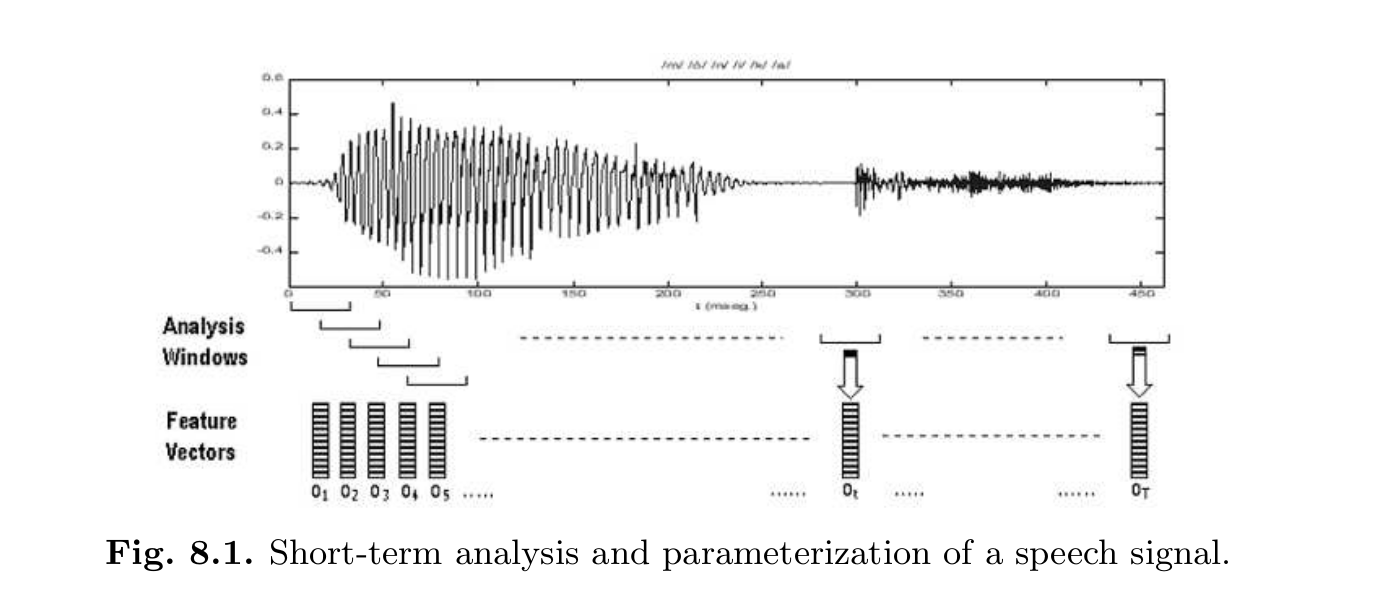
\includegraphics[width=1\linewidth]{images/figure_8_1.png}
		\caption{Phân tích theo từng đoạn ngắn và tham số hóa tín hiệu giọng nói}
		\label{fig:writing-thesis}
	\end{figure}

	\subsubsection{3.2 Tham số hóa (Parameterization)}
	\qquad Tín hiệu cửa sổ hamming/ hanning trong thời gian ngắn này có tất cả thông tin thời gian/ phổ mong muốn, mặc dù ở tốc độ bit cao (ví dụ: số hóa giọng nói điện thoại với tần số lấy mẫu 8 kHz trong một cửa sổ 32 ms. Có nghĩa là 256 mẫu x 16 bit / mẫu = 4096 bits = 512 bytes mỗi khung hình). 
	
	Phương pháp tham số hóa
	\begin{itemize}
		\item Linear Predictive Coding (LPC) 
		\item Mel-Frequency based Cepstral Coefficients (MFCC)
	\end{itemize}
	\textbf{Linear Predictive Coding (LPC)}
	\begin{figure}[H]
		\centering
		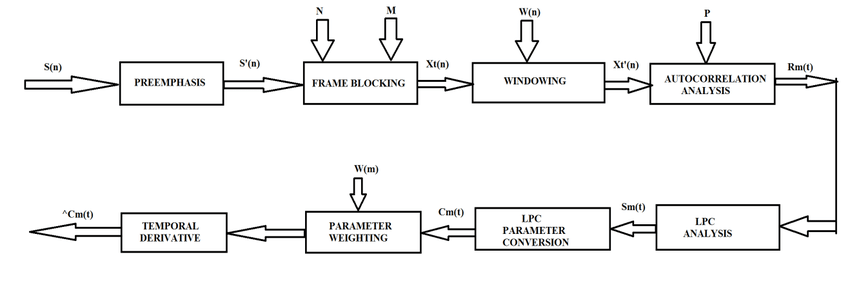
\includegraphics[width=1\linewidth]{images/Block-diagram-of-LPC-Linear-Predictive-Coding.png}
		\caption{Linear Predictive Coding (LPC) Diagram}
		\label{fig:writing-thesis}
	\end{figure}

	Linear Predictive Coding là một phương pháp sử dụng chủ yếu trong xử lý tín hiệu âm thanh và lời nói cho kết quả là đường bao phổ (đường cong đường bao của phổ biên độ - mô tả một điểm trong thời gian) của một số tín hiệu giọng nói dưới dạng nén, sử dụng thông tin của một mô hình dự đoán tuyến tính.

	\textbf{Mel-Frequency based Cepstral Coefficients (MFCC)}
	\begin{figure}[H]
		\centering
		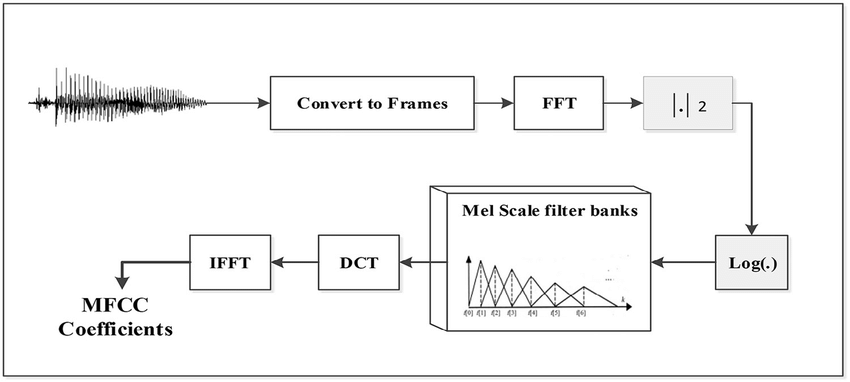
\includegraphics[width=1\linewidth]{images/Extraction-Mel-frequency-cepstral-coefficients-MFCC-from-the-audio-recording-signals.png}
		\caption{Linear Predictive Coding (LPC) Diagram}
		\label{fig:writing-thesis}
	\end{figure}

	Mel-Frequency based Cepstral Coefficients là một phương pháp để rút trích các đặc trưng (feature extraction) giọng nói thường được sử dụng trong các mô hình nhận dạng giọng nói tự động (Automatic Speech Recognition) hay phân loại giọng nói (Speech Classification).
	
	\subsubsection{3.4 Phân tách ngữ điệu (Prosodic Tokenization)}
	\qquad Các đặc trưng ngữ điệu cơ sở như cao độ và năng lượng cũng có được ở mức frame. Năng lượng cửa sổ thu được rất dễ dàng thông qua định lý Parseval, ở dạng thời gian hoặc dạng phổ, và cao độ tức thời có thể được xác định bằng, ví dụ, phương pháp tự tương quan hoặc dựa trên phân rã cepstral, thường được làm mịn bằng một số lọc thời gian.
	
	 Các đặc điểm thuận âm quan trọng khác là những đặc điểm liên quan đến thời lượng của các đơn vị ngôn ngữ, tốc độ nói và tất cả những đặc điểm liên quan đến trọng âm. 
	 
	 Trong tất cả những trường hợp đó, cần phải phân đoạn chính xác, đánh dấu các vị trí âm tiết, đường nét năng lượng và cao độ để phát hiện các vị trí trọng âm và dấu chuyển cụm từ hoặc giọng nói. 
	 
	 Việc phân đoạn ngữ âm và âm tiết của lời nói là một vấn đề phức tạp còn lâu mới giải quyết được và mặc dù nó có thể hữu ích cho việc nhận dạng giọng nói, các hệ thống âm tiết không phải lúc nào cũng yêu cầu phân đoạn chi tiết như vậy.
	
	\subsection{4. Nhận dạng giọng nói phụ thuộc văn bản}
	
	\qquad Hệ thống nhận dạng giọng nói phụ thuộc văn bản, sử dụng nội dung từ vựng của giọng nói phát ra để nhận dạng giọng nói, ứng dụng chính của hệ thống này trong các hệ thống tương tác, nơi cần có sự hợp tác từ người dùng để xác thực danh tính của họ.
	
	Ví dụ điển hình của các ứng dụng này là xác thực bằng giọng nói qua điện thoại cho các hệ thống phản hồi giọng nói tương tác yêu cầu một số mức độ bảo mật như các ứng dụng ngân hàng hoặc đặt lại mật khẩu. 
	
	Tương tự như các phương thức sinh trắc học khác, việc sử dụng hệ thống nhận dạng giọng nói phụ thuộc vào văn bản yêu cầu giai đoạn đăng ký trong đó người dùng cung cấp một số mẫu để xây dựng mô hình người dùng và giai đoạn nhận dạng trong đó mẫu giọng nói mới được so khớp với mô hình người dùng.
		
	\subsubsection{4.1 Phân loại các hệ thống và kỹ thuật}
	\qquad Chúng ta có thể phân loại hệ thống nhận dạng người nói phụ thuộc vào văn bản theo quan điểm ứng dụng thành hai loại: \textbf{hệ thống văn bản tĩnh} và \textbf{hệ thống văn bản động}. 
	
	Trong các \textbf{hệ thống văn bản tĩnh}, nội dung từ vựng trong ghi danh và các mẫu nhận dạng luôn giống nhau. Trong các \textbf{hệ thống văn bản động}, nội dung từ vựng trong mẫu nhận dạng là khác nhau trong mọi thử nghiệm truy cập với nội dung từ vựng của các mẫu đăng ký.
	
	\textbf{Hệ thống văn bản động} linh hoạt hơn và mạnh mẽ hơn trước các cuộc tấn công sử dụng bản ghi âm từ người dùng hoặc bắt chước sau khi nghe người nói thực sự nói đúng mật khẩu. Một khả năng thú vị là việc tạo ra một lời nhắc mật khẩu được tạo ngẫu nhiên khác nhau mỗi khi người dùng được xác minh (hệ thống nhắc bằng văn bản), do đó hầu như không thể sử dụng bản ghi. Đối với các kỹ thuật được sử dụng để nhận dạng người nói phụ thuộc vào văn bản, đã chứng minh rằng thông tin hiện diện ở các cấp độ khác nhau của tín hiệu giọng nói (các đặc trưng kích thích tối đa, phổ và siêu phân đoạn) có thể được sử dụng một cách hiệu quả để xác minh danh tính của người dùng. 
	
	Tuy nhiên, thông tin được sử dụng rộng rãi nhất là nội dung \textbf{phổ của tín hiệu tiếng nói}, được xác định bởi cấu hình vật lý và động lực của đường thanh quảng. Thông tin này thường được tóm tắt dưới dạng chuỗi thời gian của các vector MFCC, mỗi vector trong số đó đại diện cho một thời lượng nói từ 20-40 mili giây. Bằng cách này, vấn đề nhận dạng người nói phụ thuộc vào văn bản được giảm xuống thành vấn đề so sánh chuỗi các vector MFCC với mô hình của người dùng. 
	
	Có hai phương pháp đã được sử dụng rộng rãi: \textbf{phương pháp dựa trên khuôn mẫu} và \textbf{phương pháp thống kê}. Trong các phương pháp dựa trên khuôn mẫu mô hình của người nói bao gồm một số chuỗi vectơ tương ứng với lời nói đăng ký và việc nhận dạng được thực hiện bằng cách so sánh lời nói xác minh với lời nói đăng ký. So sánh này được thực hiện bằng cách sử dụng Dynamic Time Warping (DTW) như một cách hiệu quả để cải thiện sai lệch thời gian giữa các cách phát âm khác nhau. 
	
	Đối với các hệ thống nhúng có tài nguyên rất hạn chế, các phương pháp thống kê và đặc biệt là \textbf{Mô hình Markov ẩn (HMM)}, có xu hướng được sử dụng thường xuyên hơn các mô hình dựa trên khuôn mẫu. HMMs cung cấp tính linh hoạt hơn, cho phép chọn đơn vị tiếng nói từ đơn vị âm vị phụ đến từ và cho phép thiết kế hệ thống nhắc văn bản.
	
	\subsubsection{4.2 Kho ngữ liệu}
	\begin{itemize}
		\item YOHO Speaker Verification
		\item MIT Mobile Device Speaker Verification Corpus
		\item BIOSEC Baseline Corpus
	\end{itemize}
	
	\subsubsection{4.3 Công trình điển hình}
	\textbf{Tên công trình} Text-dependent speaker recognition with HMM speaker adaptation and HMM reestimation 
	
	Hệ thống nhận dạng giọng nói phụ thuộc văn bản được thử nghiệm trên cơ sở dữ liệu chuẩn YOHO, hai hệ thống nhận dạng người nói phụ thuộc vào văn bản do các tác giả phát triển. Các hệ thống này mô phỏng một hệ thống được nhắc bằng văn bản dựa trên một tập hợp các HMM ngữ âm không phụ thuộc vào người nói và không phụ thuộc vào ngữ cảnh được đào tạo trên TIMIT.
	
	Giai đoạn đăng ký sử dụng một số câu của người nói để điều chỉnh HMM cho người đó. Ta so sánh hai cách thức thực hiện sự thích ứng này: Baum-Welch Reestimation và MLLR (maximum likelihood linear regression).
	Trong đó, Baum-Welch Reestimation là cách tiếp cận thông thường nhất nhưng yêu cầu sử dụng HMM rất đơn giản (chỉ một hoặc một vài Gaussian cho mỗi trạng thái) còn MLLR thì mới hơn và cho phép sử dụng các HMM phức tạp hơn.
	
	Một vấn đề quan trọng trong việc phát triển hệ thống nhận dạng giọng nói phụ thuộc văn bản là số lượng tài nguyên huấn luyện. YOHO chứa 4 phần với 24 câu nói mỗi phần, đây là một lượng tài nguyên đáng kể để huấn luyện một cách hiệu quả.
	
	\begin{figure}[H]
		\centering
		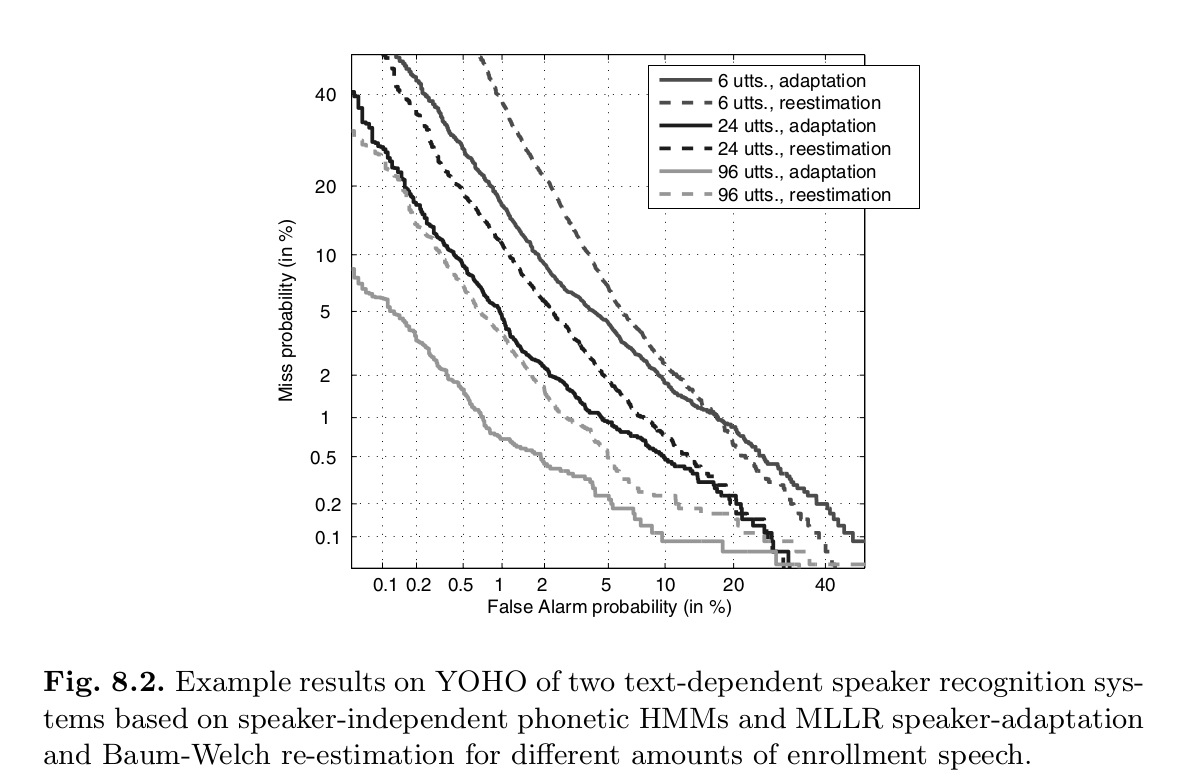
\includegraphics[width=1\linewidth]{images/figure_8_2.png}
		\caption{Linear Predictive Coding (LPC) Diagram}
		\label{fig:writing-thesis}
	\end{figure}
		
	\subsection{5. Nhận dạng giọng nói độc lập với văn bản}
	\qquad Hệ thống nhận dạng giọng nói độc lập với văn bản cố gắng giảm thiểu ảnh hưởng của nội dung từ vựng vốn được coi là không xác định đối với khả năng nhận dạng của giọng nói, điều này trái ngược với hệ thống nhận dạng giọng nói phụ thuộc văn bản, đương nhiên việc nghiên cứu và phát triển nó sẽ khó khăn hơn.
	
	\subsubsection{5.1 Short-term spectral systems}
	\qquad Khi phân tích phổ trong khoảng thời gian ngắn được sử dụng để mô hình các đặc trưng người nói, chúng ta đang mô hình hóa các “âm thanh” khác nhau mà một người có thế tạo ra, nhờ vào đường âm và các cơ quan cấu âm của họ. Khi con người cần nhiều âm thanh (hoặc các ký hiệu âm học khác nhau) để nói bằng bất kỳ ngôn ngữ chung nào, chúng ta rõ ràng đang đối mặt với một \textbf{không gian đa lớp gồm nhiều đặc trưng}.
	
	Kỹ thuật Lượng tử hóa Vector (\textbf{Vector Quantization techniques}) hiệu quả trong các bài toán đa lớp như vậy và đã được sử dụng để xác định người người, điển hình là một mô hình VQ cụ thể cho một người nói, tính toán khoảng cách từ bất kỳ câu nói nào đến bất kỳ mô hình nào dưới dạng tổng trong số của khoảng cách tối tiểu trên mỗi khung đến codevector gần của codebook. Việc sử dụng các giới hạn và các điểm trung tâm thay vì dùng mật độ xác suất làm hiệu suất của VQ kém hơn so với mô hình Markov ẩn với mật độ liên tục và liên thông hay còn gọi là Ergodic HMMs. 
	
	Tuy nhiên, yếu tố quan trọng trong \textbf{E-HMM} là tích số trạng thái với hàm Gaussian mỗi trạng thái, điều này loại bỏ triệt để ảnh hưởng của quá trình chuyển đổi trong mô hình liên thông. Sau đó, một hệ thống HMM với 5 trạng thái - 4 Gaussian cho mỗi trạng thái sẽ hoạt động tương tự như 4-trạng thái 5-Gaussian, 2-trạng thái 10-Gaussian, hoặc thậm chí là 1-trạng thái 20-Gaussian,  mà một cách hiểu tổng quát là GMM (\textbf{Gaussian Mixture Model}). Những one-state \textbf{E-HMMs} hoặc \textbf{GMMs} này có lợi thế lớn, tránh được cả ước lượng Baum-Welch cho việc huấn luyện, không cần sự liên kết giữa lời nói và trạng thái (tất cả lời nói đều được tinh chỉnh với cùng một trạng thái duy nhất) và dùng Viterbi decoding cho việc việc kiểm thử (không cần tinh chỉnh thời gian), giúp tăng tốc thời gian tính toán mà không ảnh hưởng đến hiệu suất.
	
	\textbf{GMM} là một kỹ thuật tổng hợp trong đó một hỗn hợp các hàm Gaussians Đa chiều cố gắng mô hình hóa phân phối thống kê chưa rõ của dữ liệu người nói. GMM trở thành một kỹ thuật hiện đại vào những năm 1990, cả khi \textbf{Maximum likehood} (Tối đa hóa kỳ vong \textbf{Expectation-Maximization}, EM) hoặc huấn luyện phân loại (\textbf{Maximum Mutual Information}, MMI) còn được dùng. Tuy nhiên, việc sử dụng MAP tương thích với hầu hết phương tiện từ một \textbf{Universal Background Model} (UBM) đã mang lại cho GMMs một lợi thế lớn so với các kỹ thuật khác, đặc biệt khi được sử dụng với các kỹ thuật chuẩn hóa như \textbf{Z-standar}d (chuẩn hóa điểm giả), \textbf{T-norm} (chuẩn hóa âm thanh), \textbf{H-norm} (chuẩn Z phụ thuộc vào thiết bị cầm tay), \textbf{HT-norm} (H + T-norm) hoặc \textbf{Feature Mapping} (xác định và chuẩn hóa kênh).
	
	\textbf{Discriminative techniques} - Kỹ thuật phân tách như \textbf{Artificial Neural Networks}, đã được sử dụng trong nhiều năm, nhưng hiệu suất của chúng chưa bao giờ đạt đến hiệu suất của \textbf{GMM}. Tuy nhiên, vào cuối những năm 90, \textbf{SVM - Support Vector Machine} được ví như một bộ phân loại hiệu năng cao được huấn luyện sẵn, mang lại cho \textbf{GMM} một đối thủ cạnh tranh vì hiệu suất gần như tương đương bằng việc sử dụng \textbf{SVM} trong không gian nhiều chiều hơn với các kernel tích hợp như GLDS (\textbf{Generalized Linear Discriminant Sequence Kernel})
	
	Gần đây, việc sử dụng \textbf{SuperVectors}, một kỹ thuật hỗn hợp \textbf{GMM-SVM} coi là công cụ của \textbf{GMM} cho mọi trường hợp (cả trong huấn luyện và kiểm tra) là các điểm trong không gian nhiều chiều (số chiều bằng với số hỗn hợp của \textbf{GMM} nhân với số chiều của vector được tham số hóa) bằng cách sử dụng \textbf{SVM} cho mỗi người nói để phân loại các cách phát âm chưa biết từ siêu phẳng giọng nói được huấn luyện sẵn.
	
	\subsubsection{5.2 Idiolectal systems (Idiolectal = idio (personal, private) + (dia)lect)}
	\qquad Hầu hết hệ thống nhận dạng người nói không phụ thuộc văn bản đều dựa vào đặc trưng phổ ngắn cho đến khi công trình của Doddington được công bố, nó mở ra một thế giới mới khả năng cải thiện các hệ thống nhận dạng người nói không phụ thuộc vào văn bản. 
	
	Doddington đã nhận ra và chứng minh rằng lời nói của những người nói khác nhau không chỉ khác nhau về âm học, mà còn về các đặc điểm khác như cách sử dụng từ. Đặc biệt, trong công việc của mình, ông đã lập mô hình cách sử dụng từ của từng người nói cụ thể bằng cách sử dụng \textbf{n-gram} mô hình hóa các chuỗi từ và xác suất của chúng và chứng minh rằng việc sử dụng các mô hình đó có thể cải thiện hiệu suất của hệ thống GMM âm thanh/ phổ cơ bản. Quan trọng hơn kết quả cụ thể này là thực tế là công trình này đã thúc đẩy nghiên cứu trong việc sử dụng các cấp độ thông tin cao hơn (idiolectal, phonotactic, prosodic, v.v.) để \textbf{nhận dạng giọng nói độc lập với văn bản}. 
	
	Các phần tiếp theo mô tả hai trong số những hệ thống thành công nhất khai thác mức độ thông tin cao hơn: hệ thống âm vị, cố gắng mô hình hóa các đặc điểm phát âm và hệ thống thuận âm, mô hình hóa các mẫu âm thanh chuyên biệt dành cho người nói.
	
	\subsubsection{5.3 Phonotactic systems}
	\qquad Một hệ thống nhận dạng giọng nói phonotactic điển hình bao gồm hai khối chính:
	\begin{itemize}
		\item Bộ giải mã ngữ âm (the phonetic decoders), chuyển đổi lời nói thành một chuỗi các nhãn ngữ âm.
		\item Giai đoạn mô hình hóa ngôn ngữ thống kê n-gram, mô hình hóa tần số của ngữ âm và chuỗi ngữ âm cho mỗi người nói cụ thể.
	\end{itemize}

	\begin{figure}[H]
		\centering
		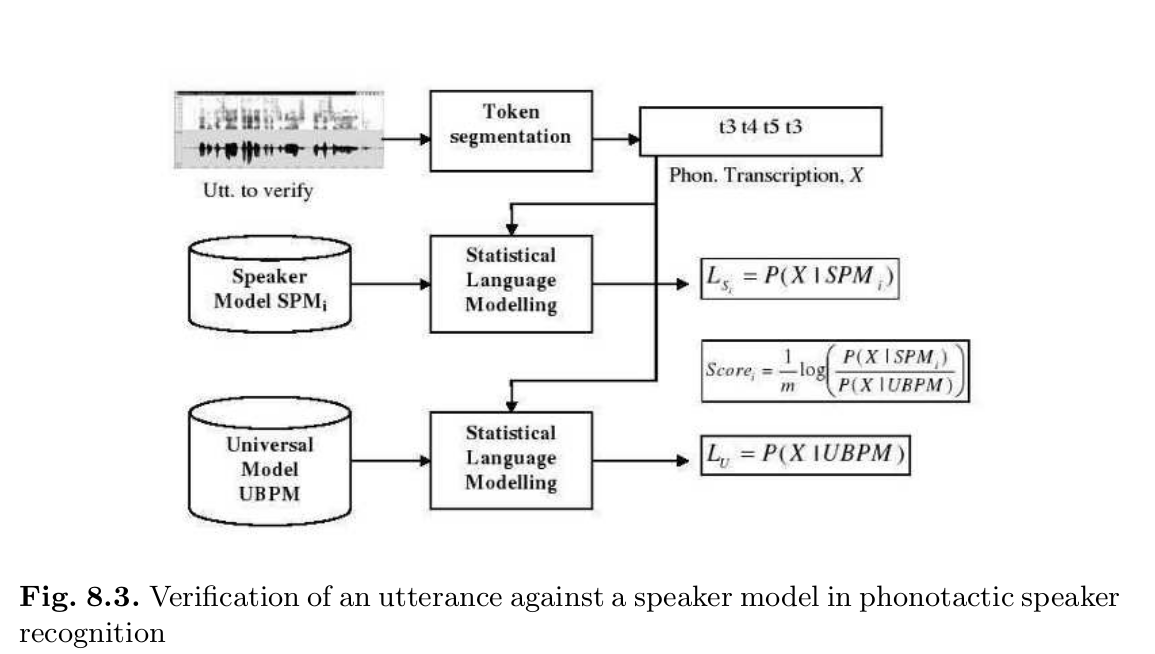
\includegraphics[width=1\linewidth]{images/figure_8_3.png}
		\caption{Quy trình của hệ thống ngữ âm}
		\label{fig:writing-thesis}
	\end{figure}
	
	\textbf{Bộ giải mã ngữ âm} – thường dựa trên \textbf{Mô hình Markov ẩn (HMMs)} - có thể được lấy từ trình nhận dạng giọng nói có sẵn hoặc được huấn luyện đặc biệt. Đối với mục đích nhận dạng người nói, việc có bộ giải mã ngữ âm không quan trọng và thậm chí không quan trọng lắm phải có bộ giải mã ngữ âm trong ngôn ngữ của người nói để được nhận dạng. Thực tế có phần đáng ngạc nhiên này đã được phân tích cho thấy rằng các lỗi ngữ âm phụ thuộc vào giọng nói do bộ giải mã tạo ra dường như là của giọng nói cụ thể và do đó thông tin hữu ích cho việc nhận dạng giọng nói miễn là các lỗi này phù hợp với từng giọng nói cụ thể.
	
	Sau khi có bộ giải mã ngữ âm, bản giải mã ngữ âm của nhiều câu từ nhiều giọng nói khác nhau có thể được sử dụng để huấn luyện \textbf{Mô hình Universal Background Phone} ($UBPM$) đại diện cho tất cả những giọng nói có thể có. Các \textbf{Mô hình Ngữ âm Giọng nói} ($SPM_i$ - \textbf{Speaker Phone Models}) được huấn luyện bằng cách sử dụng một số bộ giải mã ngữ âm của từng người nói cụ thể. Vì giọng nói có sẵn để huấn nói một mô hình giọng nói thường bị hạn chế, các mô hình giọng nói được nội suy với $UBPM$ để tăng tính mạnh mẽ trong ước tính tham số. 
	
	Sau khi các mô hình ngôn ngữ thống kê được huấn luyện, quy trình để xác minh cách phát âm một tập test so với mô hình giọng nói $SPM_i$ được trình bày trong Hình 8.3. Bước đầu tiên là tạo ra giải mã ngữ âm của nó, $X$, giống như cách giải mã được sử dụng để huấn luyện $SPM_{i}$ và $UBPM$. Sau đó, giải mã ngữ âm của câu thử, $X$ và các mô hình thống kê ($SPM_{i}$, UBPM) được sử dụng để tính toán khả năng giải mã ngữ âm, $X$, dựa trên mô hình giọng nói $SPM_{i}$ và mô hình nền $UBPM$. 
	
	\textbf{Điểm nhận dạng là logarith tỷ lệ của cả hai khả năng xảy ra}. Quá trình này, thường được mô tả là Nhận dạng ngữ âm, sau đó là Mô hình hóa ngôn ngữ ($PRLM$) có thể được lặp lại cho các bộ giải mã ngữ âm khác nhau (ví dụ: các ngôn ngữ hoặc độ phức tạp khác nhau) và các điểm nhận dạng khác nhau chỉ được thêm vào hoặc hợp nhất để có hiệu suất tốt hơn, mang lại một phương pháp được gọi là $PRLM$ hoặc $PPRLM$ song song. Gần đây, một số cải tiến đã được đề xuất trên các hệ thống $PPRLM$ cơ bản. 
	
	Một trong những điều quan trọng nhất về mặt cải thiện hiệu năng là việc sử dụng toàn bộ mạng lưới nhận dạng ngữ âm thay vì giả thuyết rằng có một bộ giải mã tốt nhất. Mạng lưới nhận dạng là một đồ thị không chu trình có hướng chứa các giả thuyết có khả năng xảy ra nhất cùng với các xác suất của chúng. Thông tin phong phú hơn nhiều này cho phép ước tính tốt hơn \textbf{n-gam} trên các tài nguyên giọng nói hạn chế, và do đó cho kết quả tốt hơn nhiều. Cải tiến quan trọng khác là việc sử dụng \textbf{SVM} để phân lớp toàn bộ n-gam được huấn luyện với giả thuyết tốt nhất hoặc với mạng thay vì sử dụng chúng trong framework phân lớp thống kê.
	
	\textbf{Tóm tắt các bước hoạt động của mô hình}
	\begin{itemize}
		\item Bước 1: Đầu vào là giọng nói cần xác minh
		\item Bước 2 - Token segmentation: Tách thành các đoạn t3, t4, t5, t3
		\item Bước 3: Mô hình hóa ngôn ngữ thống kê n-gram
		\begin{itemize}
			\item Huấn luyện mô hình Universal Background Phone (UBPM) $L_{U} = P(X|UBPM)$
			\item Huấn luyện mô hình Speaker Phone Models ($SPM_{i}$): $L_{S_{i}} = P(X | SPM_{i})$
		\end{itemize}
		\item Bước 4: Tính recognition score: $Score_{i} = \frac{1}{m}log\left(\frac{P(X | SPM_{i})}{P(X|UBPM)}\right)$
	\end{itemize}

	\begin{figure}[H]
		\centering
		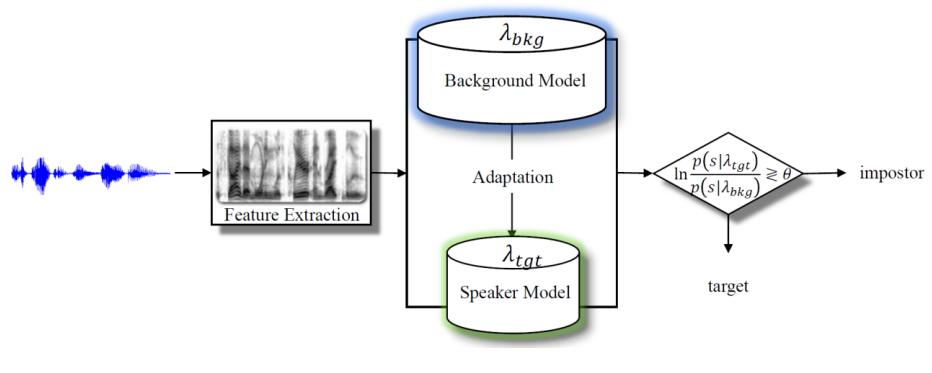
\includegraphics[width=1\linewidth]{images/diagram.png}
		\caption{Quy trình của hệ thống ngữ âm}
		\label{fig:writing-thesis}
	\end{figure}
	
	\subsubsection{5.4 Prosodic systems}
	\qquad Một trong những hệ thống ngữ điệu tiên phong và thành công nhất trong việc nhận dạng giọng nói không phụ thuộc vào văn bản là công trình của Adami. Hệ thống bao gồm hai khối xây dựng chính: 
	\begin{itemize}
		\item Phân tách ngữ điệu, phân tích ưu điểm và biểu thị nó dưới dạng một chuỗi các nhãn hoặc token
		\item Mô hình hóa ngôn ngữ thống kê n-gram, mô hình hóa tần số của các tokens và trình tự của từng giọng nói cụ thể
	\end{itemize}
	 
	 Một số khả năng khác để mô hình hóa thông tin ngữ điệu cũng đã được chứng minh là khá thành công là việc sử dụng Non-uniform Extraction Region Features (NERFs) được phân định bằng khoảng dừng đủ dài hoặc NERF được xác định bởi cấu trúc âm tiết của câu (SNERFs).
	
	Các tác giả đã triển khai một hệ thống ngữ điệu dựa trên công trình của Adami, trong đó khối thứ hai giống hệt nhau để nhận dạng ngữ âm và âm sắc chỉ với những điều chỉnh nhỏ để cải thiện hiệu suất. Quá trình tokenization bao gồm hai giai đoạn:
	\begin{itemize}
		\item Giai đoạn một, đối với mỗi đoạn giọng nói của đoạn thoại, quỹ đạo thời gian của các đặc điểm thuận (tần số cơ bản - hoặc cao độ- và năng lượng) được rút trích
		\item Giai đoạn hai, cả hai đường bao đều được phân đoạn và dán nhãn bằng định lượng trung bình độ dốc.
	\end{itemize}

	\begin{figure}[H]
		\centering
		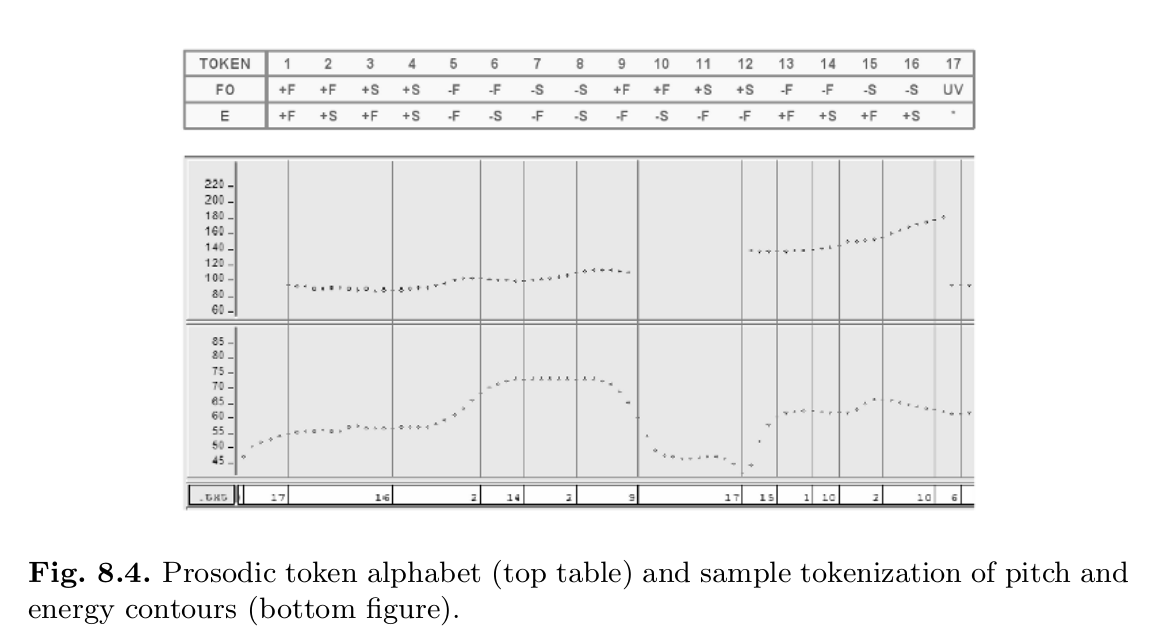
\includegraphics[width=1\linewidth]{images/figure_8_4.png}
		\caption{Token ngữ điệu alphabet}
		\label{fig:writing-thesis}
	\end{figure}

	Hình trên là một bảng chứa 17 token ngữ điệu. Một token đại diện cho các phân đoạn vô thanh, trong khi 16 token được sử dụng để đại diện cho các phân đoạn hữu thanh tùy thuộc vào độ dốc (phát nhanh, tăng chậm, giảm nhanh, giảm chậm) của năng lượng và cao độ.
	
	\subsubsection{5.5 Cơ sở dữ liệu và benchmarks}
	\begin{itemize}
		\item Vào năm 1996, NIST bắt đầu Đánh giá Nhận dạng Giọng nói -Speaker Recognition Evaluations hàng năm, đây chắc chắn là động lực của những tiến bộ đáng kể.
		\item Các hội thảo sau đánh giá đã cho phép người tham gia chia sẻ kinh nghiệm, cải tiến, thất bại, v.v. của họ trong một môi trường hợp tác cao. Vai trò của LDC (Linguistic Data Consortium) cung cấp tài liệu nói mới đầy thách thức cũng rất đáng chú ý, vì nhu cầu liên tục tăng lên (cả về lượng lời nói và yêu cầu ghi âm)
		\item Các bộ đánh giá trước đây (phát triển, huấn luyện và kiểm tra âm thanh và chìa khóa giải pháp) có sẵn thông qua LDC - Linguistic Data Consortium để các nhà nghiên cứu mới đánh giá hệ thống của họ mà không có áp lực cạnh tranh
	\end{itemize}
	
	\subsubsection{5.6 Công trình điển hình}
	\textbf{Tên công trình}: The ATVS multilevel text-independent system
	\begin{figure}[H]
		\centering
		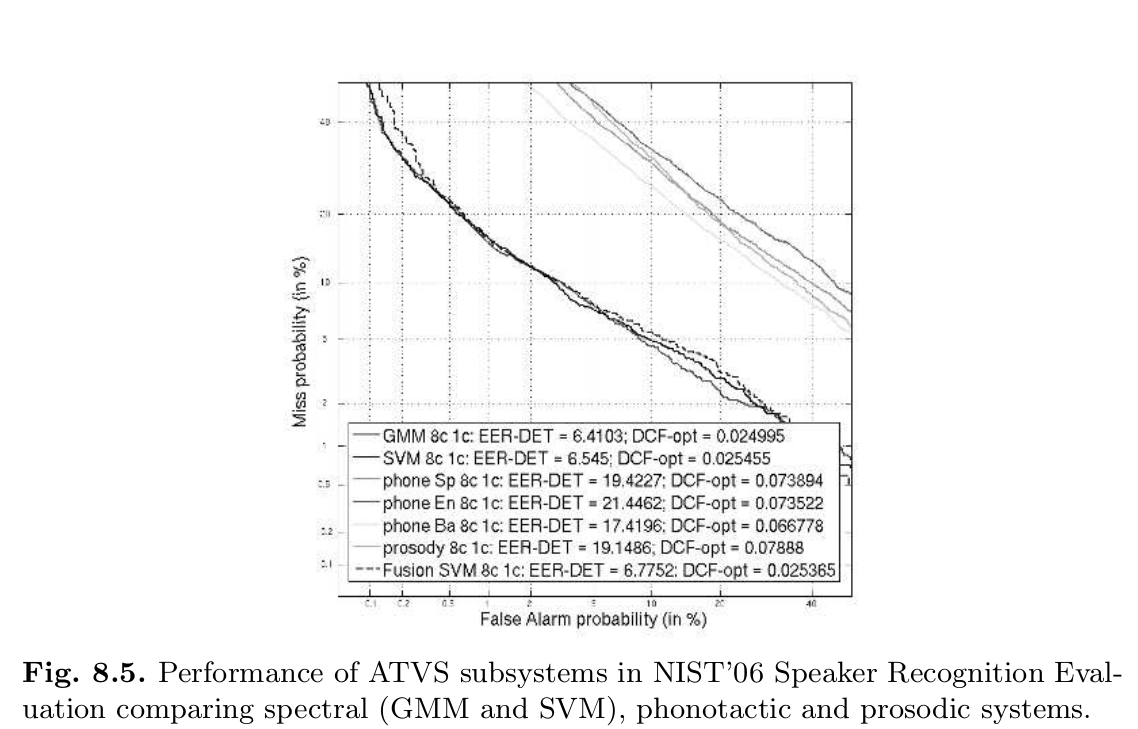
\includegraphics[width=1\linewidth]{images/figure_8_5.png}
		\caption{Linear Predictive Coding (LPC) Diagram}
		\label{fig:writing-thesis}
	\end{figure}

	Kết quả tại NIST SRE06 trong nhiệm vụ 8c1c (8 conversation for training và 1 conversation for testing), để xem hiệu suất của các hệ thống con khác nhau trên cùng một bài tập. Sự khác biệt chính của hệ thống ATVS năm 2006 so với hệ thống 2005 là việc sử dụng Ánh xạ đặc trưng trong cả GMM và SVM, việc sử dụng mở rộng đa thức bậc 3 (thay vì bậc 2) trong nhân GLDS và việc sử dụng của một PRLM được huấn luyện với SpeechDat
	
	\begin{figure}[H]
		\centering
		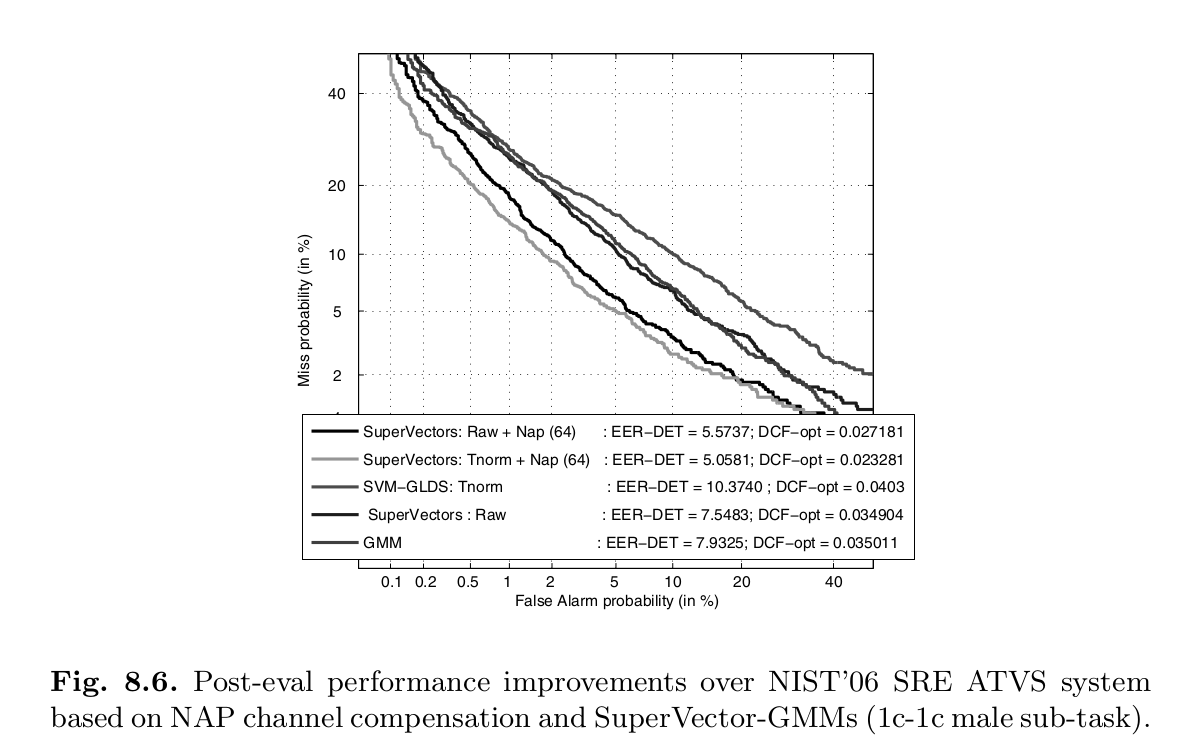
\includegraphics[width=1\linewidth]{images/figure_8_6.png}
		\caption{Linear Predictive Coding (LPC) Diagram}
		\label{fig:writing-thesis}
	\end{figure}

	\section{D.2 Các phương pháp SOTA - State of The Art trong Voice Biometrics}
	\subsection{D.2.1 Giới thiệu}
	
	\subsection{D.2.2 Động lực nghiên cứu}
	
	\subsection{D.2.3 Phát biểu bài toán}
	\textbf{Tác vụ:} Định danh người nói
	\begin{itemize}
		\item Đầu vào (Input): Dữ liệu âm thanh giọng nói
		\item Đầu ra (Output): Danh tính của người nói
	\end{itemize}
	\textbf{Tác vụ:} Xác nhận người nói
	\begin{itemize}
		\item Đầu vào (Input): Dữ liệu âm thanh giọng nói
		\item Đầu ra (Output): Đồng ý/ Từ chối
	\end{itemize}

	\subsection{D.2.4 Kho ngữ liệu}
	
	\subsection{D.2.5 Các công trình liên quan}
	Các công trình liên quan trong giai đoạn gần đây, áp dụng Học Sâu vào tác vụ nhận dạng giọng nói
	
	\subsubsection{D.2.5.1 }


	\section{E. Thực nghiệm của nhóm}
	
	\nocite{*}
	\bibliography{references}\newpage\cleardoublepage
	\bibliographystyle{plain}
	
\end{document}
